%!TEX root = ../tudkom_students__201804_v1.4.tex
\chapter{Einleitung}
%This chapter should motivate the thesis, provide a clear description of the problem to be solved, and describe the major contributions of this thesis.
% 2 pages

\section{Motivation}
%What is the motivation for doing research in this area?
Die Nachfrage nach Wearables steigt kontinuierlich.
Abbildung \ref{fig:stat_wearables} zeigt, dass sich der Absatz in den letzten vier Jahren versechsfacht hat.
Wearables sind Geräte, die am Körper getragen werden, um zum Beispiel mithilfe von Sensoren Daten zu erfassen \cite{definition_wearables}.\\
Ein weit verbreiteter Anwendungsfall ist die Herzfrequenzmessung beim Sport mit einem Fitnessarmband.
Durch das Auswerten dieser Daten kann die Trainingsintensität in Echtzeit an die Person angepasst und somit die Effektivität gesteigert werden.
\begin{figure}[h]
	\centering
	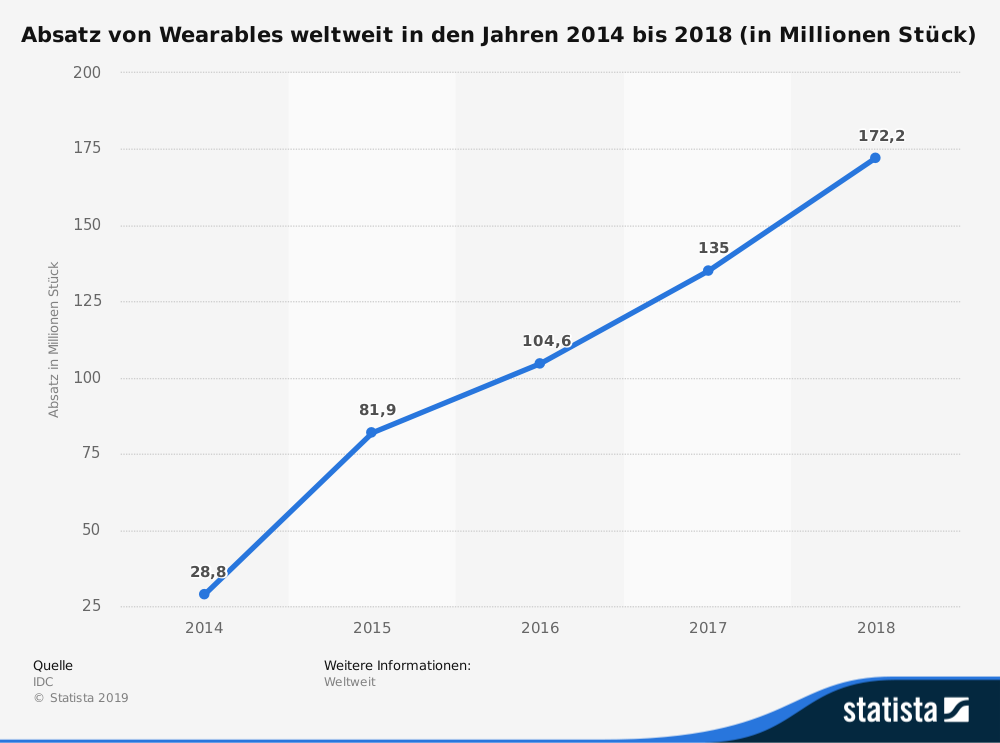
\includegraphics[width=0.75\linewidth]{res/01_statistic_id515723_absatz-von-wearables-weltweit-bis-2018.png}
	\caption{Absatz von Wearables \cite{statistik_wearables}}
	\label{fig:stat_wearables}
\end{figure}\\
In dieser Arbeit hingegen wird ein Wearable entworfen, dass die Position und Rotation von Gelenken erfasst.
Auf der Analyse dieser Daten aufbauend können dann weiterführende Anwendungsfälle entwickelt werden.
Folgende sind zum Beispiel interessante Anwendungen:
\begin{itemize}
  \item Das Erkennen von falsch ausgeführten Übungen beim Sport oder falscher Haltung beim Sitzen oder Stehen im Alltag. Dadurch können negative gesundheitliche Folgen vermieden werden.
  \item Eine Lösung für mobiles Motion Capturing zum Erstellen von Animationen in Filmen oder Videospielen. Mit der Anzahl der Wearables kann die Auflösung der Bewegung proportional zum Preis skaliert werden.
  \item Ein Echtzeitsystem zur Übersetzung von Zeichensprache in gesprochene Sprache zur Kommunikation von stummen Menschen.
  \item Für die Bewegungserkennung in Videospielen und Virtual Reality. Abbildung \ref{fig:stat_konsolen} zeigt, dass die Nintendo Wii die fünftmeistverkaufteste Konsole ist und damit die Geschichte der Videospielkonsolen prägt. Die Fernbedienung übernimmt bei ihr die gleichen Funktionen wie das hier entwickelte Wearable. Zusätzlich kann man mit dem Nunchuk einen zweiten Bewegungssensor anschließen. Das hier entwickelte Wearable könnte dieses System erweitern und weitere Vorteile bieten, zum Beispiel, dass die Hände beim Spielen frei bleiben. Bei VR-Headset werden neben Fernbedienungen wie bei der Wii auch Kameras zur Ganzkörper-Bewegungserkennung genutzt.
\end{itemize}
\begin{figure}[h]
  \centering
  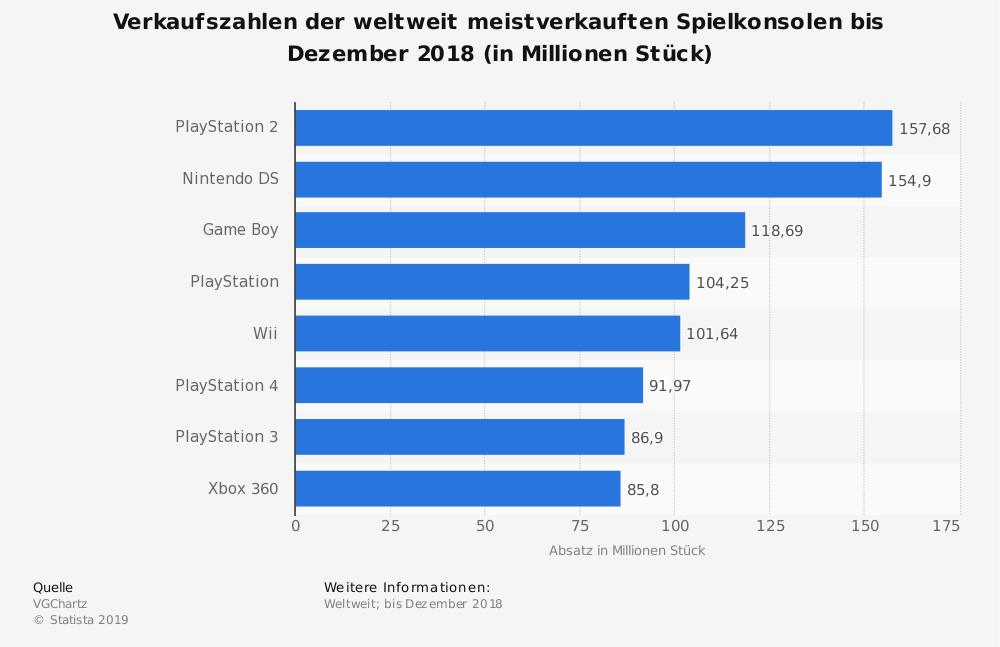
\includegraphics[width=0.75\linewidth]{res/01_statistic_id160549_weltweit-meistverkaufte-spielkonsolen-bis-dezember-2018.png}
  \caption{Verkaufszahlen der weltweit meistverkauften Spielkonsolen \cite{statistik_konsolen}}
  \label{fig:stat_konsolen}
\end{figure}

%blabla gesten auf handy erkennen blabla sport blabla auch motion capturing für videos und spiele

\section{Problem Statement and Contribution}
%What is the problem that should be solved with this thesis?
blabla welche möglichkeiten blabla welche technik/protokolle ausgewählt blabla

\section{Outline}
%How is the rest of this thesis structured?
blabla struktur
